\chapter{Graphical Representation of the Predicted Conformations}\label{appendix:visual}

\begin{figure}[ht]
    \centering
    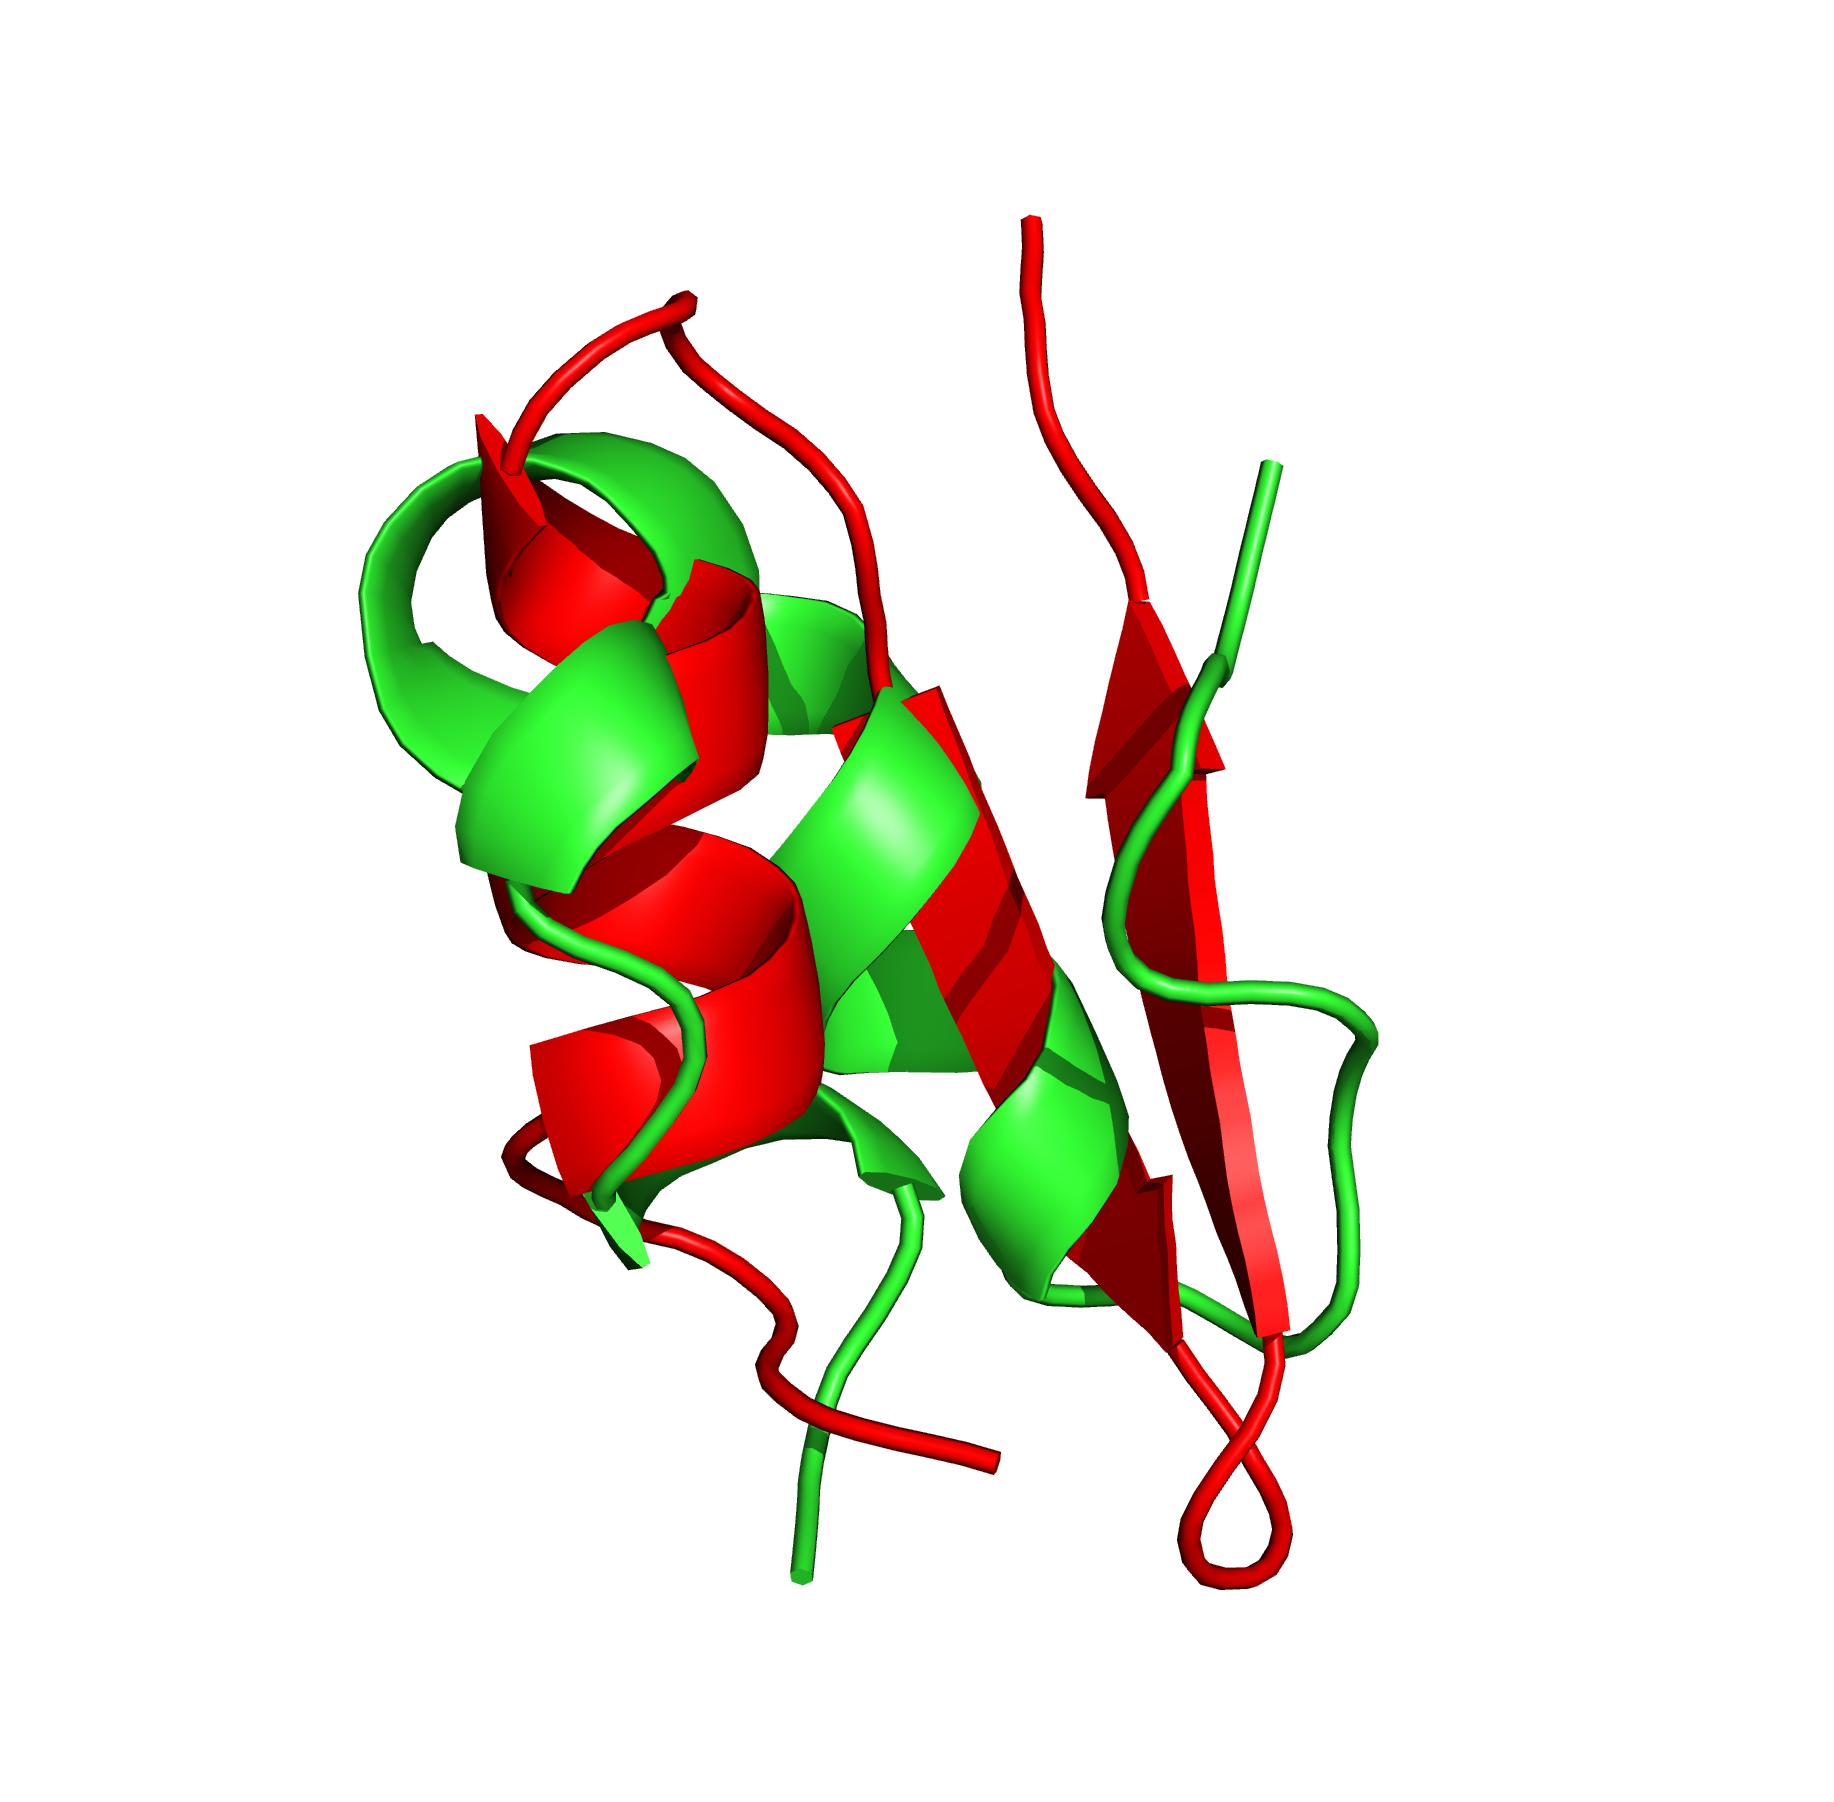
\includegraphics[width=0.9\linewidth]{Figuras/prots/1acw_render.png}
    \caption{Predicted Conformation of 1acw (green, light) over the Native Conformation}
    \label{fig:1acw-visual}
\end{figure}

\begin{figure}[ht]
    \centering
    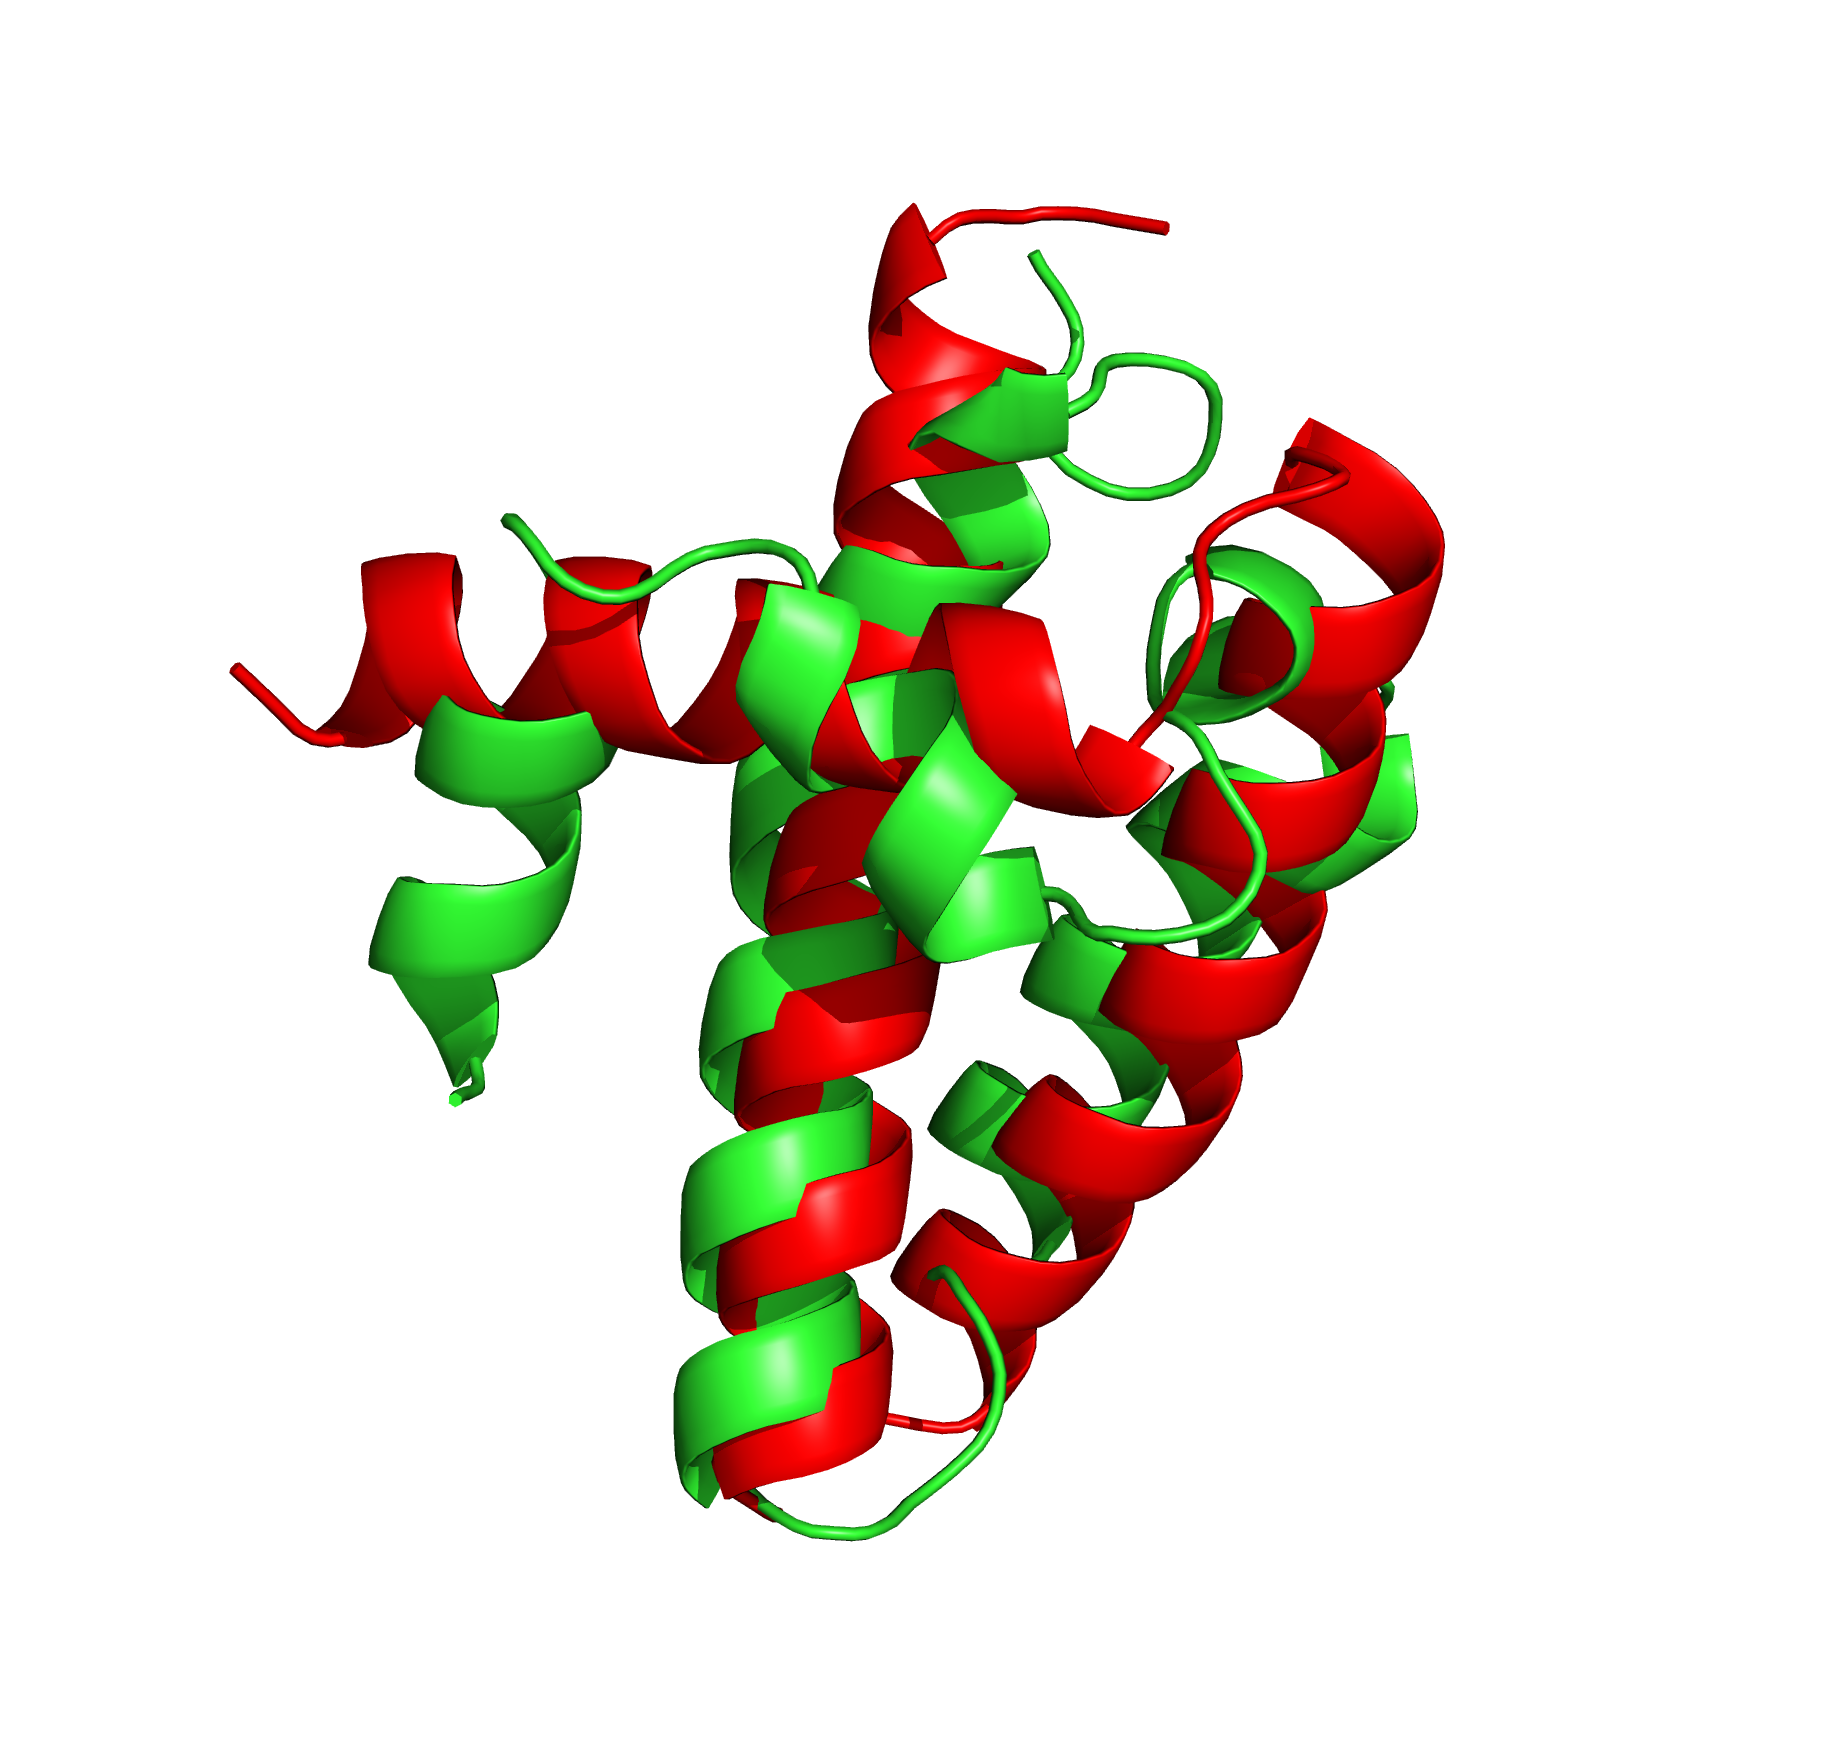
\includegraphics[width=0.9\linewidth]{Figuras/prots/1ail_render.png}
    \caption{Predicted Conformation of 1ail (green, light) over the Native Conformation}
    \label{fig:1ail-visual}
\end{figure}

\begin{figure}[ht]
    \centering
    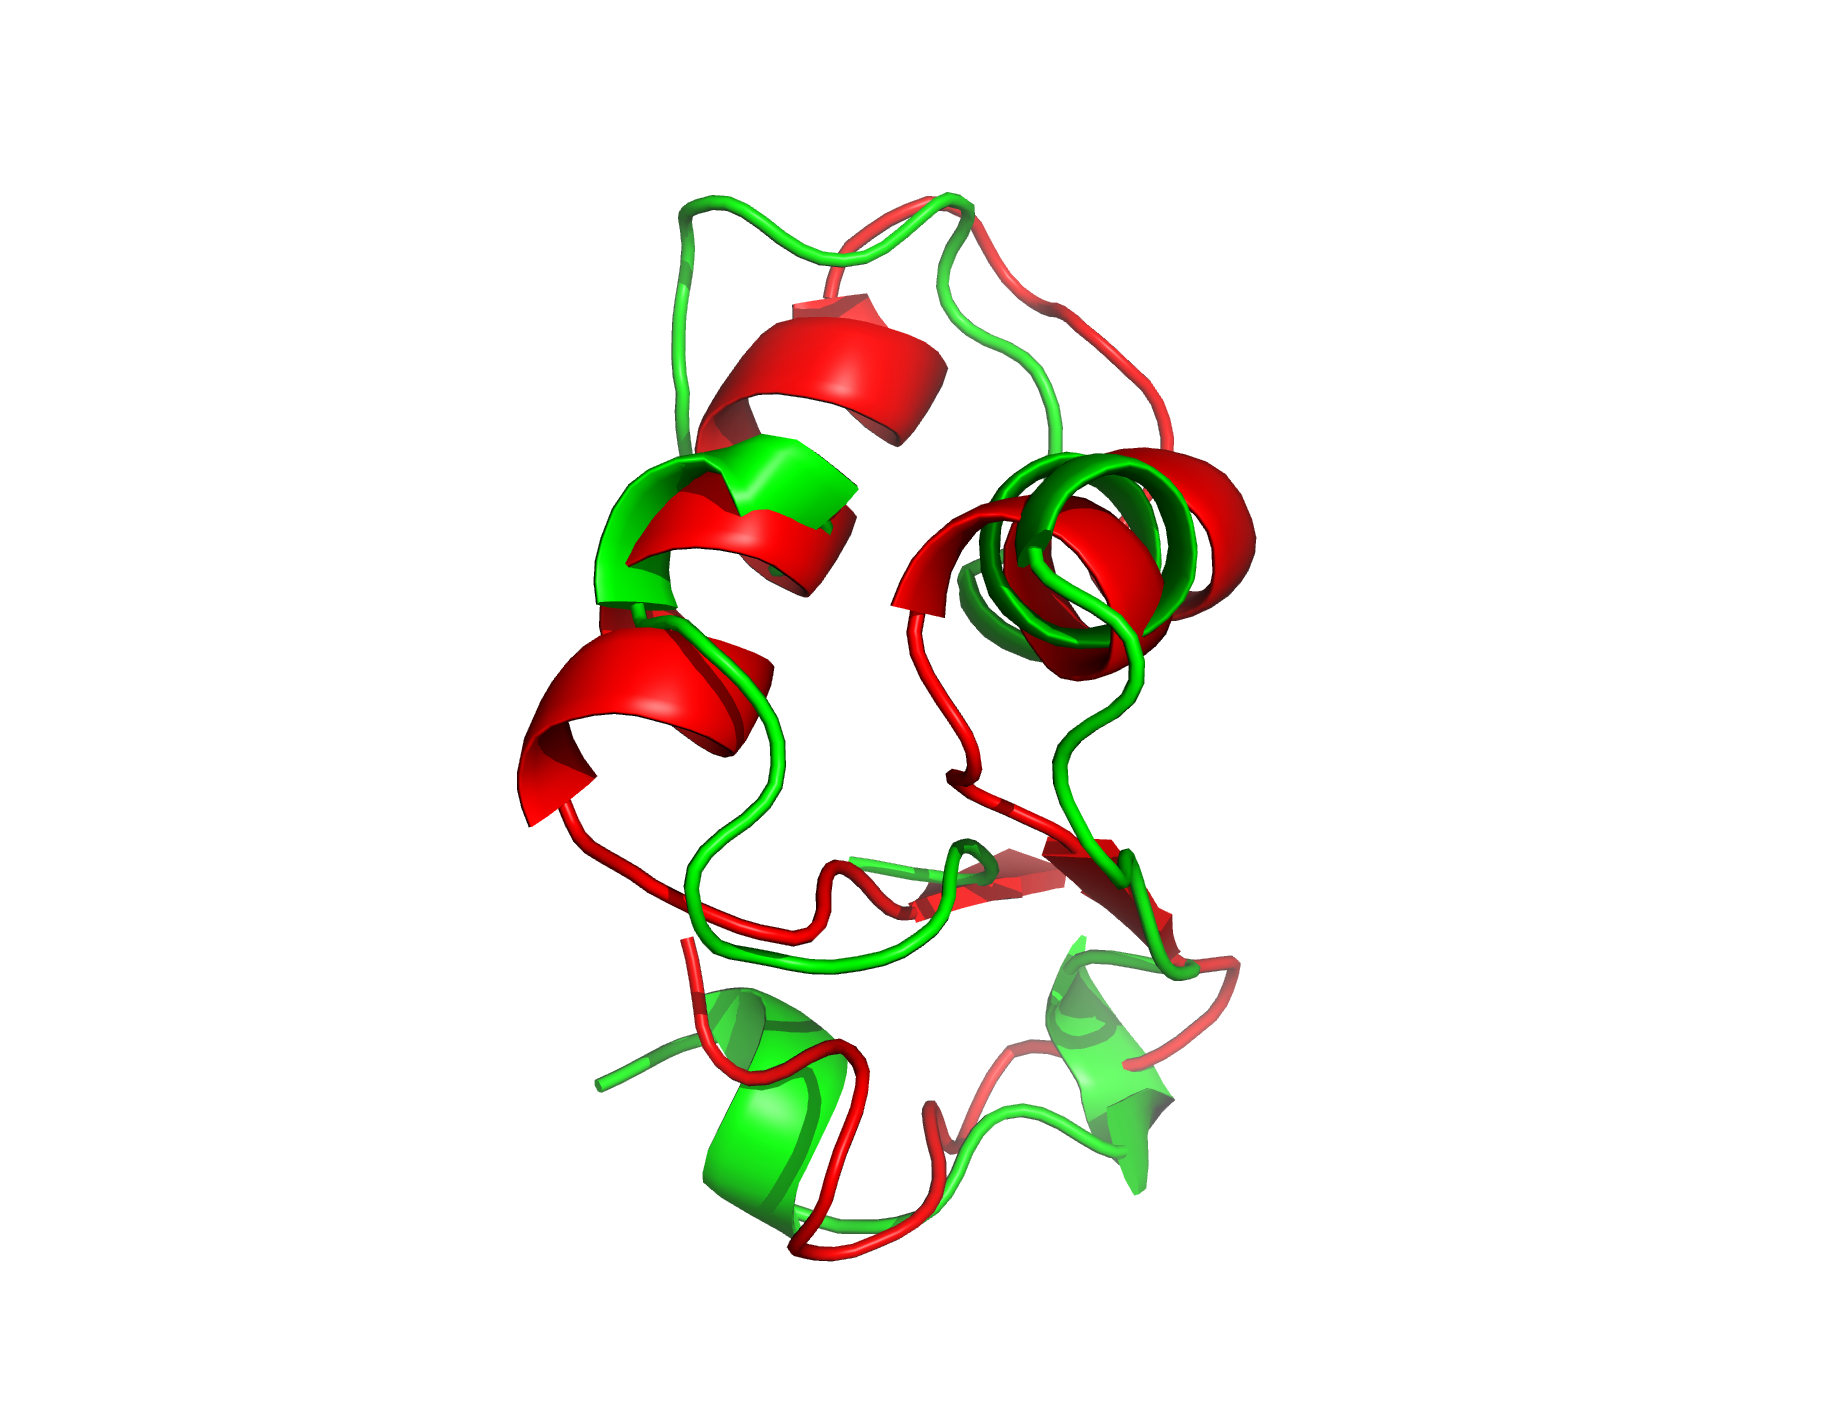
\includegraphics[width=0.9\linewidth]{Figuras/prots/1crn_render.png}
    \caption{Predicted Conformation of 1crn (green, light) over the Native Conformation}
    \label{fig:1crn-visual}
\end{figure}

\begin{figure}[ht]
    \centering
    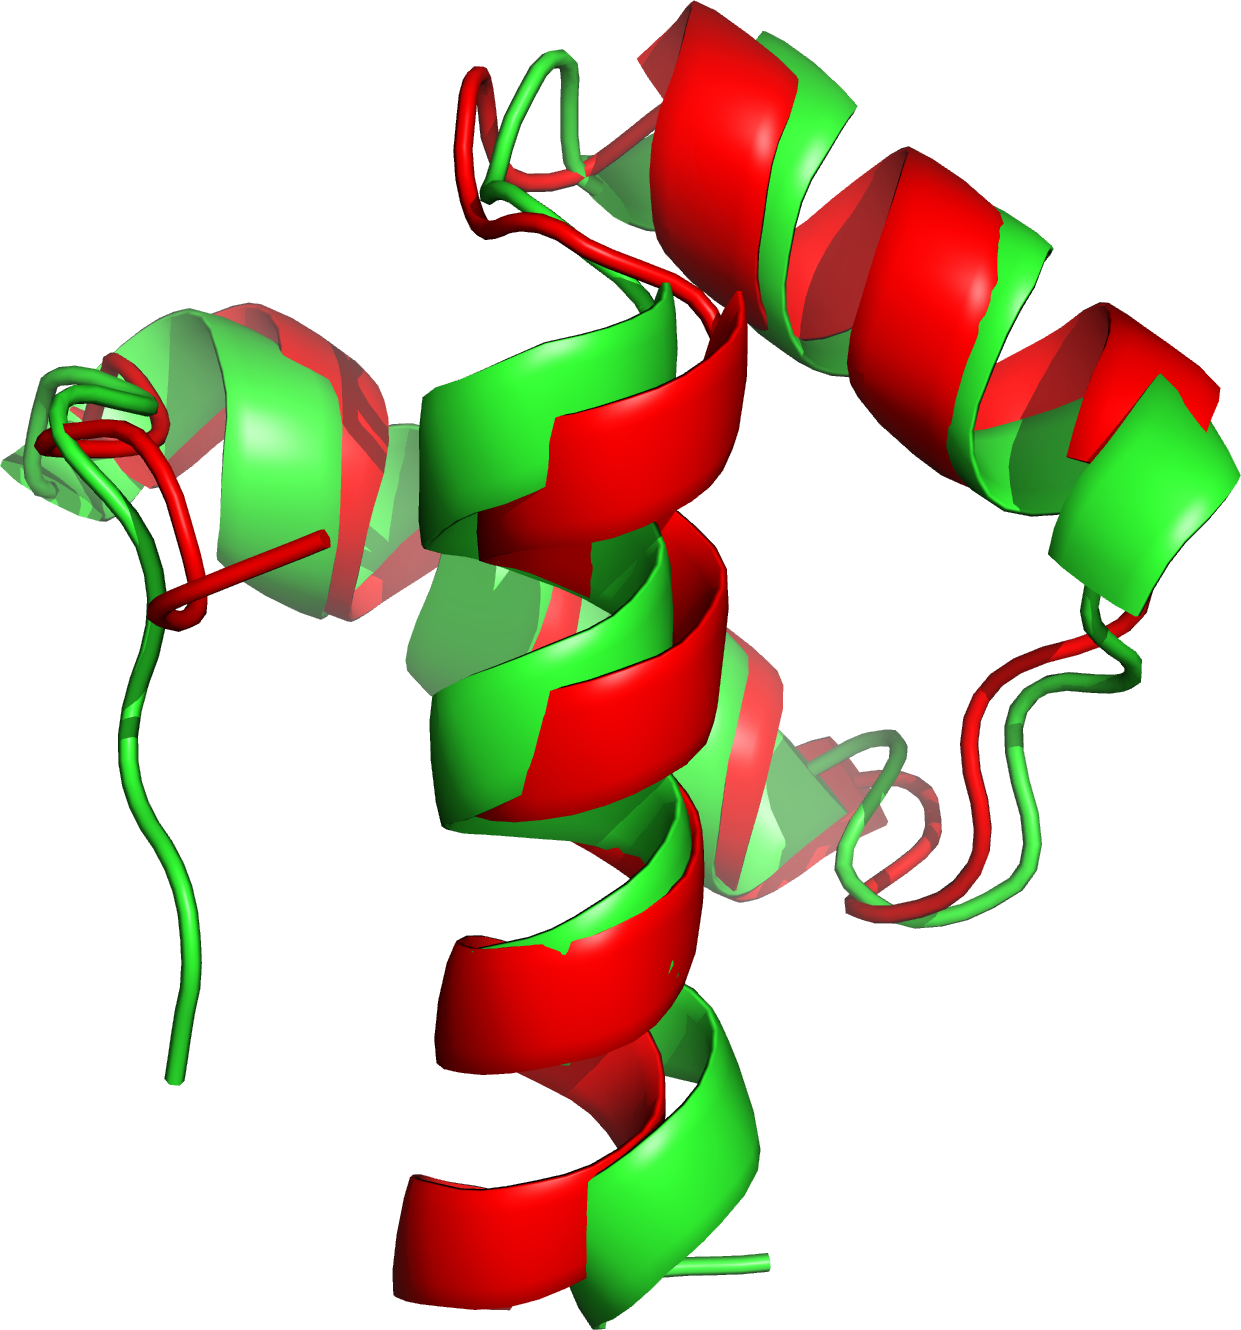
\includegraphics[width=0.9\linewidth]{Figuras/prots/1enh_render.png}
    \caption{Predicted Conformation of 1enh (green, light) over the Native Conformation}
    \label{fig:1enh-visual}
\end{figure}

\begin{figure}[ht]
    \centering
    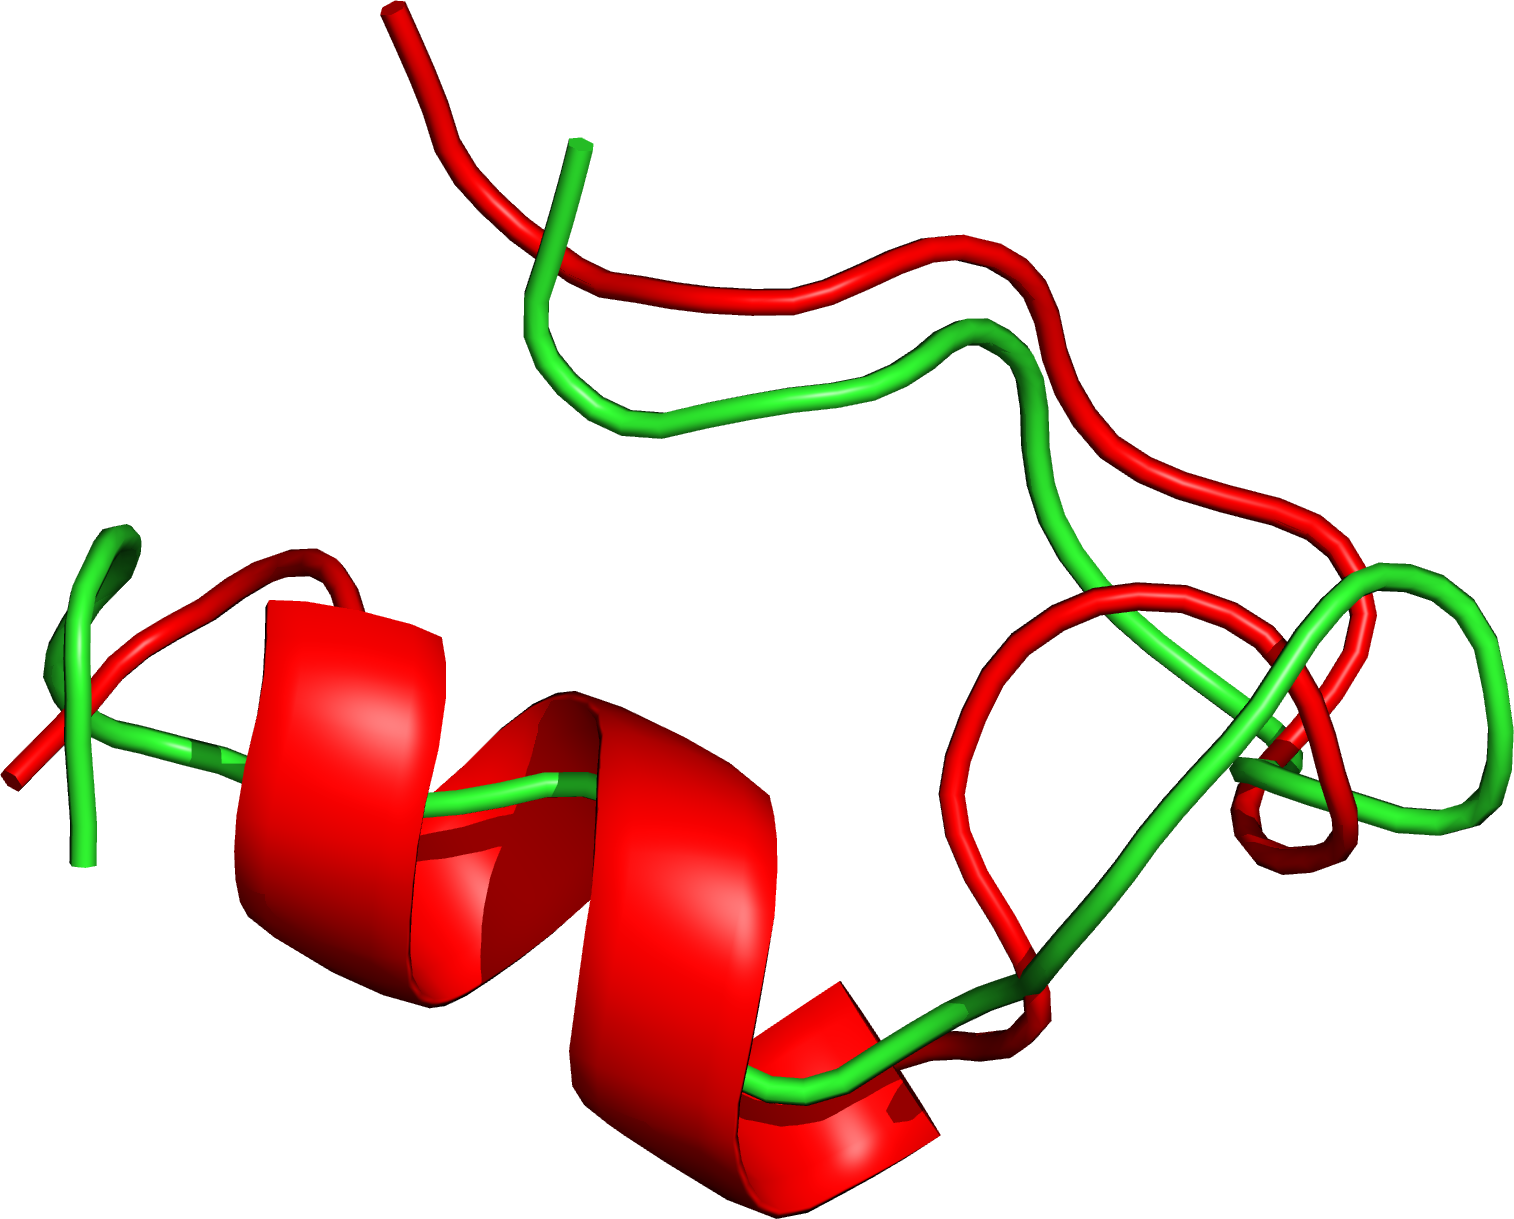
\includegraphics[width=0.9\linewidth]{Figuras/prots/1l2y_render.png}
    \caption{Predicted Conformation of 1l2y (green, light) over the Native Conformation}
    \label{fig:1l2y-visual}
\end{figure}

\begin{figure}[ht]
    \centering
    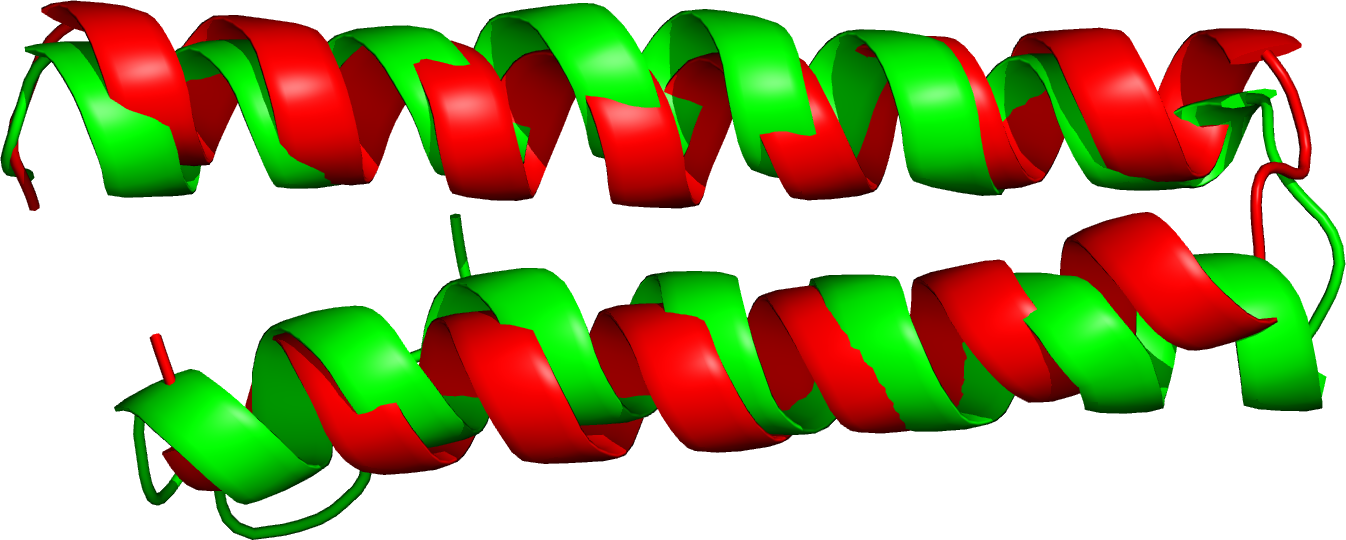
\includegraphics[width=0.9\linewidth]{Figuras/prots/1rop_render.png}
    \caption{Predicted Conformation of 1rop (green, light) over the Native Conformation}
    \label{fig:1rop-visual}
\end{figure}

\begin{figure}[ht]
    \centering
    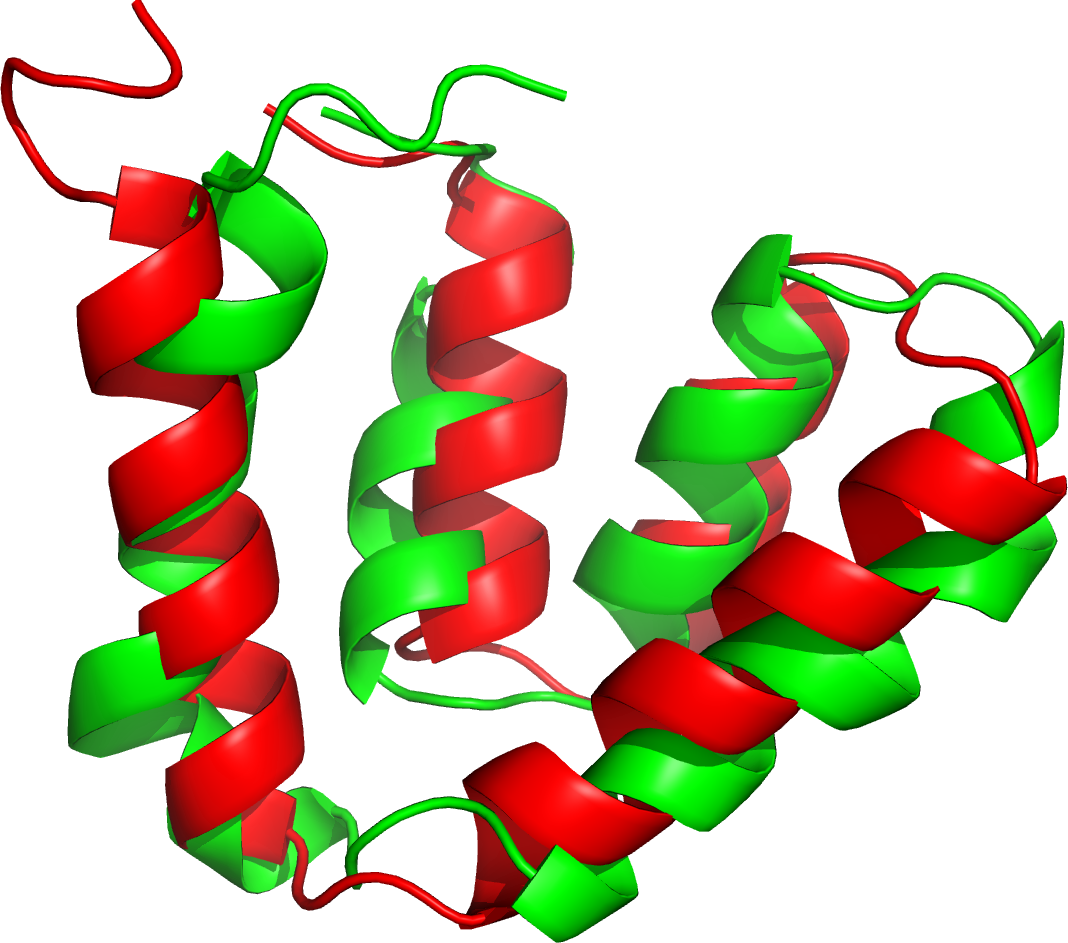
\includegraphics[width=0.9\linewidth]{Figuras/prots/1utg_render.png}
    \caption{Predicted Conformation of 1utg (green, light) over the Native Conformation}
    \label{fig:1utg-visual}
\end{figure}

\begin{figure}[ht]
    \centering
    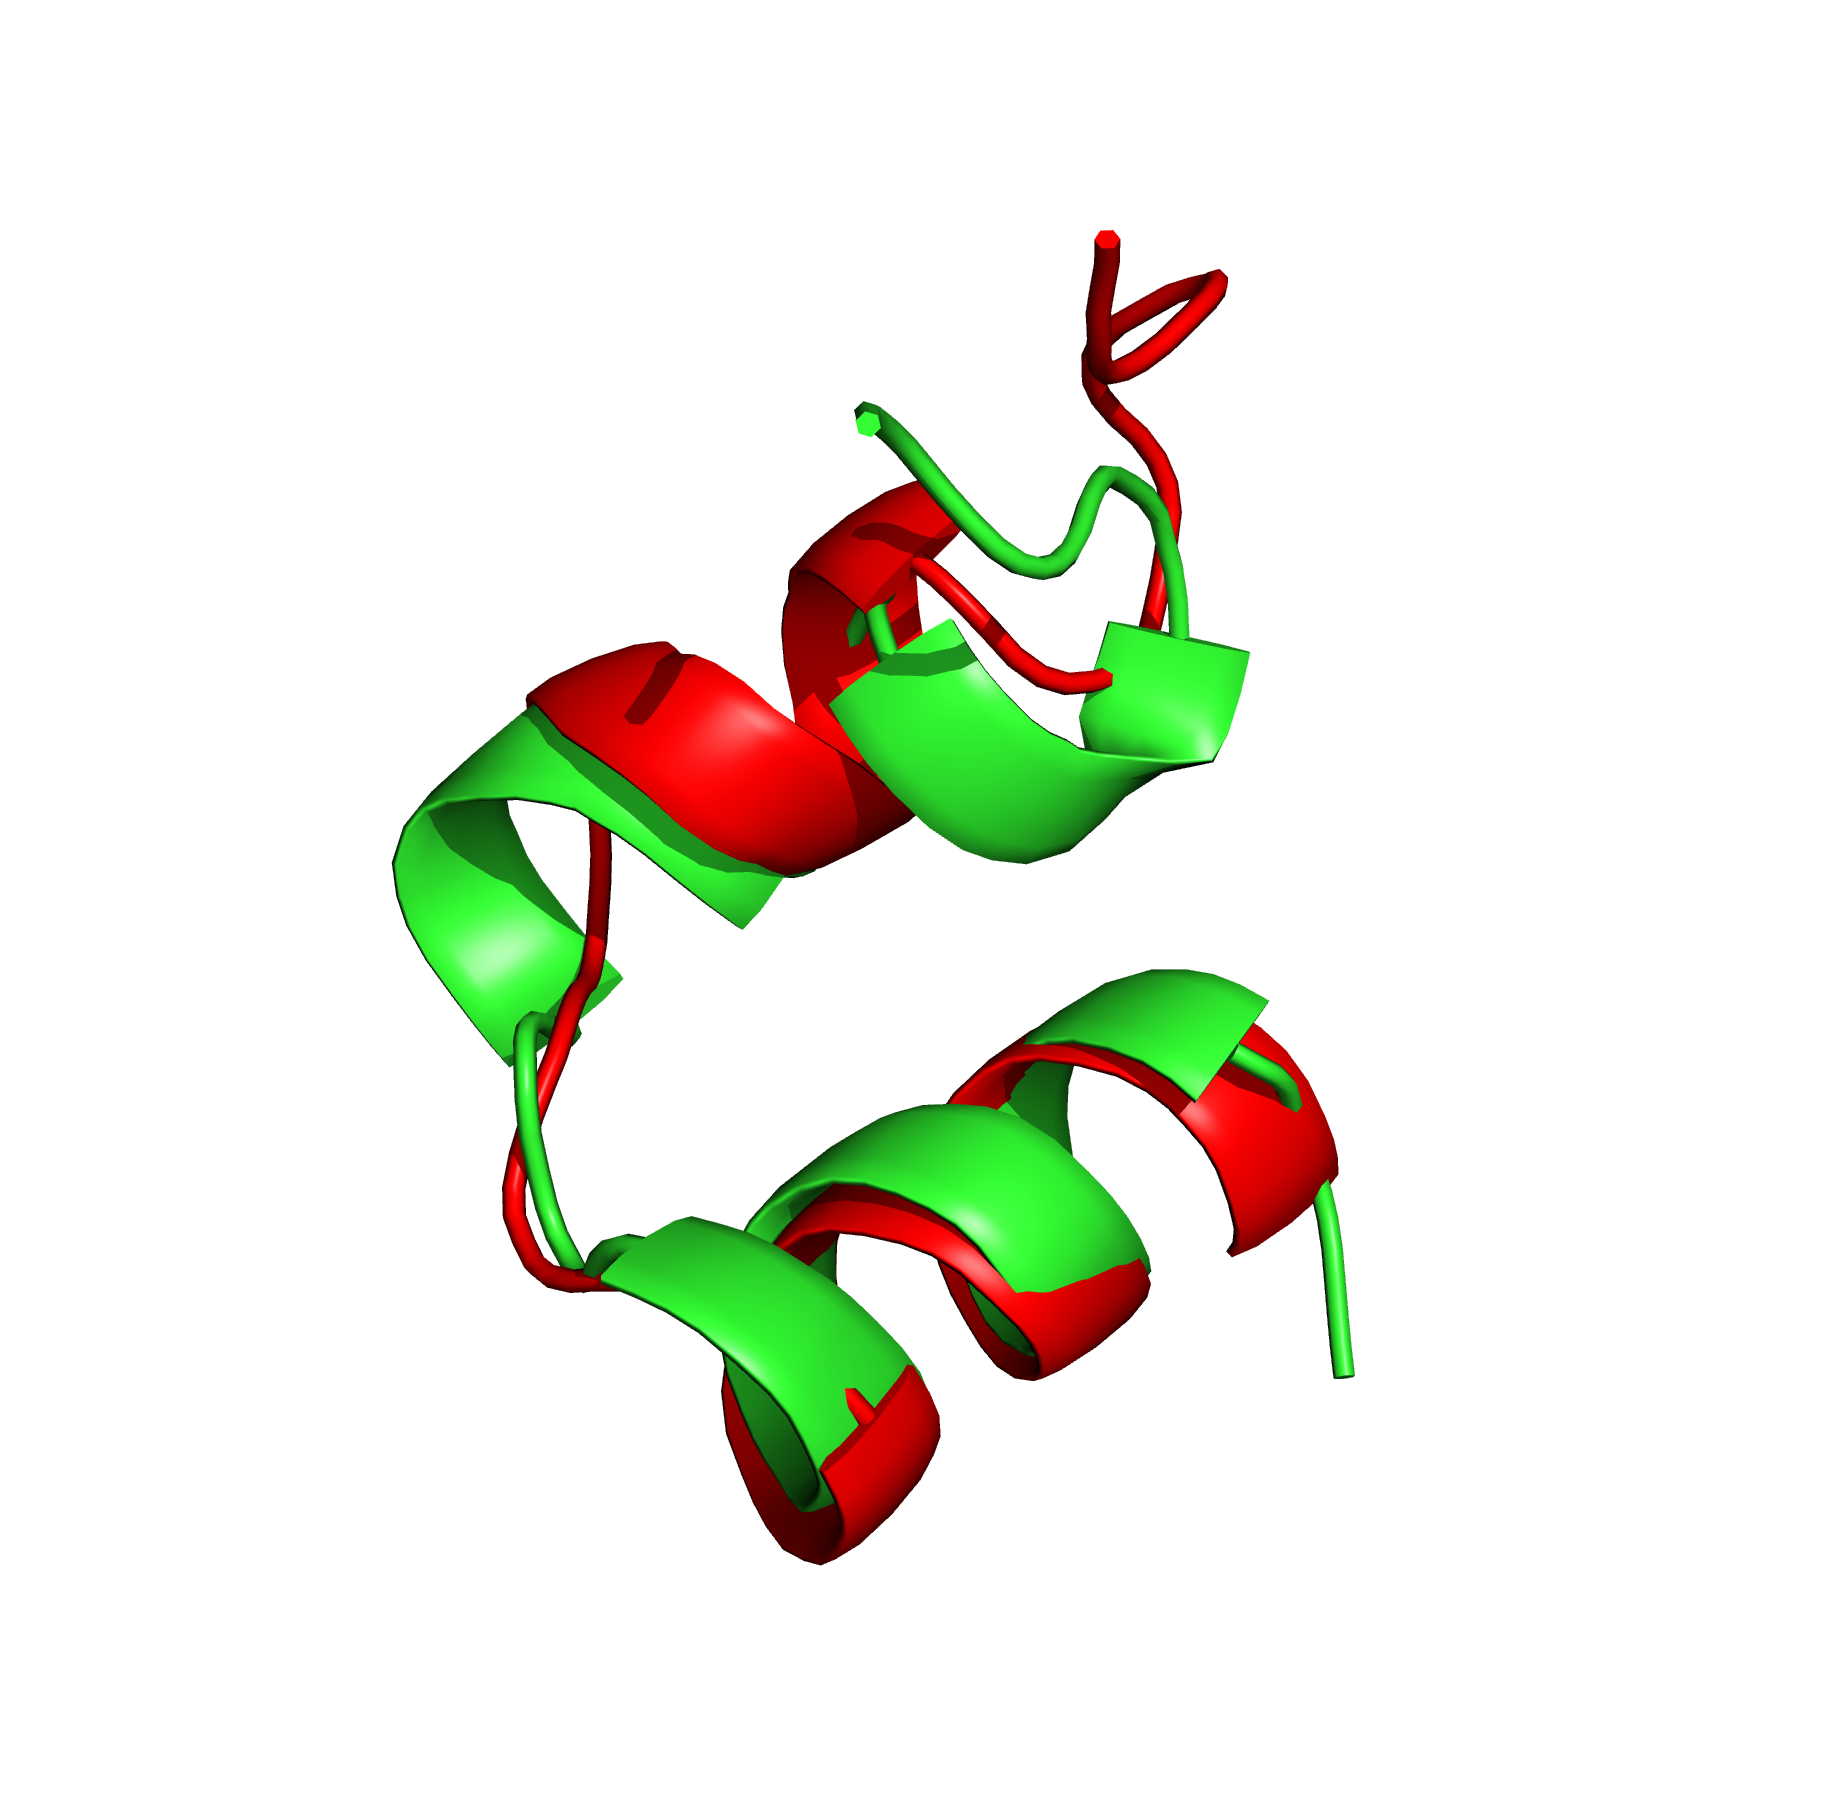
\includegraphics[width=0.9\linewidth]{Figuras/prots/1wqc_render.png}
    \caption{Predicted Conformation of 1wqc (green, light) over the Native Conformation}
    \label{fig:1wqc-visual}
\end{figure}

\begin{figure}[ht]
    \centering
    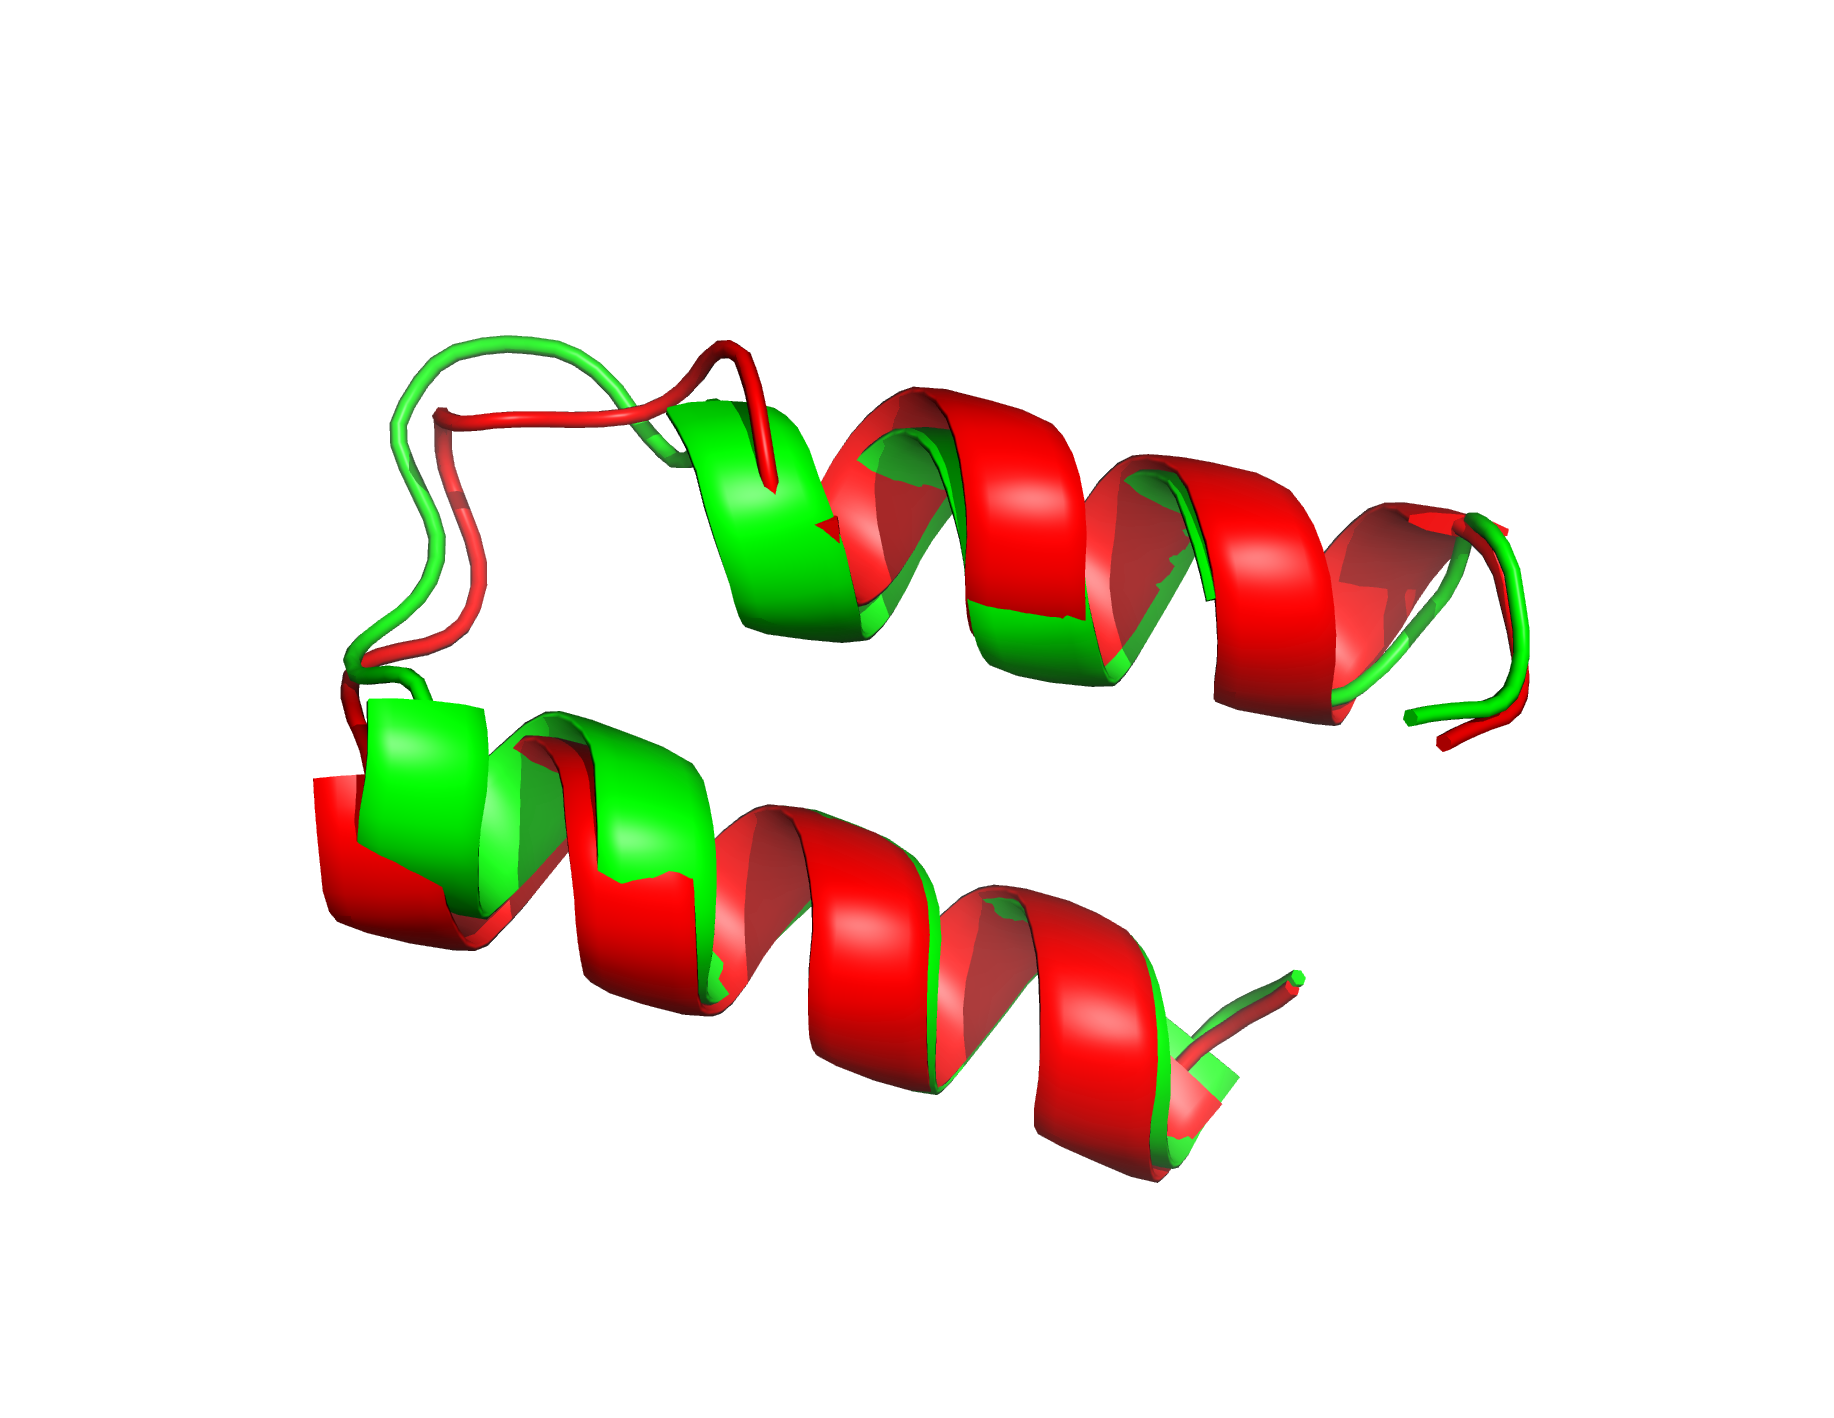
\includegraphics[width=0.9\linewidth]{Figuras/prots/1zdd_render.png}
    \caption{Predicted Conformation of 1zdd (green, light) over the Native Conformation}
    \label{fig:1zdd-visual}
\end{figure}

\begin{figure}[ht]
    \centering
    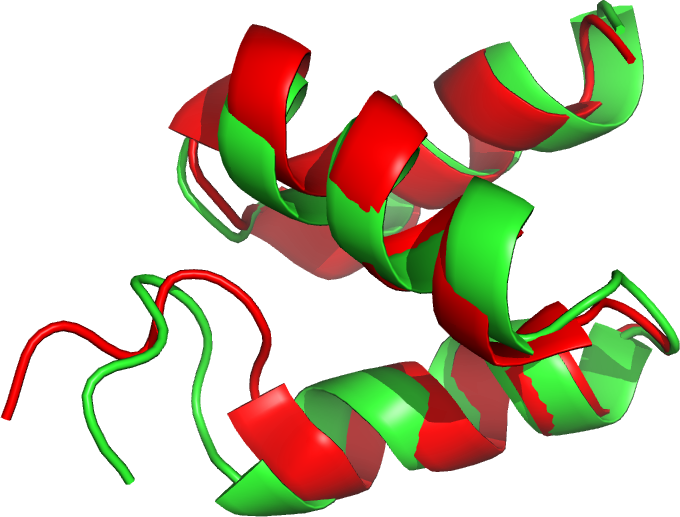
\includegraphics[width=0.9\linewidth]{Figuras/prots/2mr9_render.png}
    \caption{Predicted Conformation of 2mr9 (green, light) over the Native Conformation}
    \label{fig:2mr9-visual}
\end{figure}

